%%% Folie
{
\scriptsize

\begin{frame}{Leitfragen des heutigen Kapitels}
    \begin{block}{Aufbau der Referenzarchitektur}
        \begin{itemize}
            \setlength\itemsep{.5em}

            \item Welche Komponenten umfasst die Beispielarchitektur?
            \item Wozu werden die einzelnen Komponenten benötigt?
            \item Welche Vor- und Nachteile besitzt die Architektur?
        \end{itemize}
    \end{block}

    \begin{block}{Verwendung der Entwicklungswerkzeuge}
        \begin{itemize}
            \setlength\itemsep{.5em}

            \item Wie registriert man sich bei der Balena Cloud?
            \item Wie wird der Raspberry Pi mit der Balena Cloud verbunden?
            \item Wie lässt sich Software auf dem Raspberry Pi installieren?
            \item Wie kann man realitätsnah und dennoch einfach entwickeln?
        \end{itemize}
    \end{block}

    \begin{block}{Softwarearchitektur der Devices}
        \begin{itemize}
            \setlength\itemsep{.5em}

            \item Welche Softwarekomponenten werden benötigt?
            \item Wie flexibel ist die deviceseitige Architektur?
            \item Wie kann die Komplexität begrenzt werden?
            \item Wie können die Komponenten untereinander kommunizieren?
        \end{itemize}
    \end{block}

    \begin{block}{Kommunikation mit dem Internet}
        \begin{itemize}
            \setlength\itemsep{.5em}

            \item Wie können Sensordaten über das Internet verschickt werden?
            \item Wie kann ein Device über das Internet ferngesteuert werden?
            \item Wie lassen sich weitere Devices möglichst einfach integrieren?
        \end{itemize}
    \end{block}
\end{frame}
}

%%% Folie
{
\scriptsize

\begin{frame}{Lernziele}
    \begin{block}{IoT-Entwicklung mit der Balena Cloud}
        \begin{itemize}
            \setlength\itemsep{.5em}

            \item x
        \end{itemize}
    \end{block}

    \begin{block}{Nutzung des Redis Key-Value-Store}
        \begin{itemize}
            \setlength\itemsep{.5em}

            \item x
        \end{itemize}
    \end{block}

    \begin{block}{Datenaustausch mit MQTT}
        \begin{itemize}
            \setlength\itemsep{.5em}

            \item x
        \end{itemize}
    \end{block}
\end{frame}
}

%-------------------------------------------------------------------------------
\section{IoT-Systemarchitektur}
%-------------------------------------------------------------------------------

{
\small

%%% Folie
\begin{frame}{Definition ,,Eingebettetes Computersystem''}
    \begin{block}{Definition}
        \parbox{\linewidth}{
            \smallskip

            Eingebettete Systeme sind kleine Mikrocomputer, die innerhalb eines größeren Geräts
            meist unsichtbar verbaut sind, um seine Funktionen zu steuern und überwachen. In vielen
            Fällen geben sie einem Gerät überhaupt erst seine Funktion, ohne dass dies für den
            Anwender offensichtlich ist.
            \smallskip

            Ihre grundsätzliche Architektur ist dieselbe wie bei konventionellen Computern,
            jedoch verfügen sie über weitaus weniger, genau auf den Anwendungsfall zugeschnittene
            Ressourcen bei minimalen Kosten, Platzbedarf und Energieverbrauch. Der Leitgedanke
            hierbei lautet ,,so viel wie gerade nötig, so wenig wie absolut möglich''.
            Eingebettete Systeme sind meist in sich geschlossene Systeme mit deterministischem
            Systemverhalten, die rund um die Uhr laufen und exakt eine Aufgabe erfüllen.
        }
    \end{block}

    \begin{block}{Beispiele}
        \begin{columns}[onlytextwidth]
            \column[b]{.2\textwidth}
            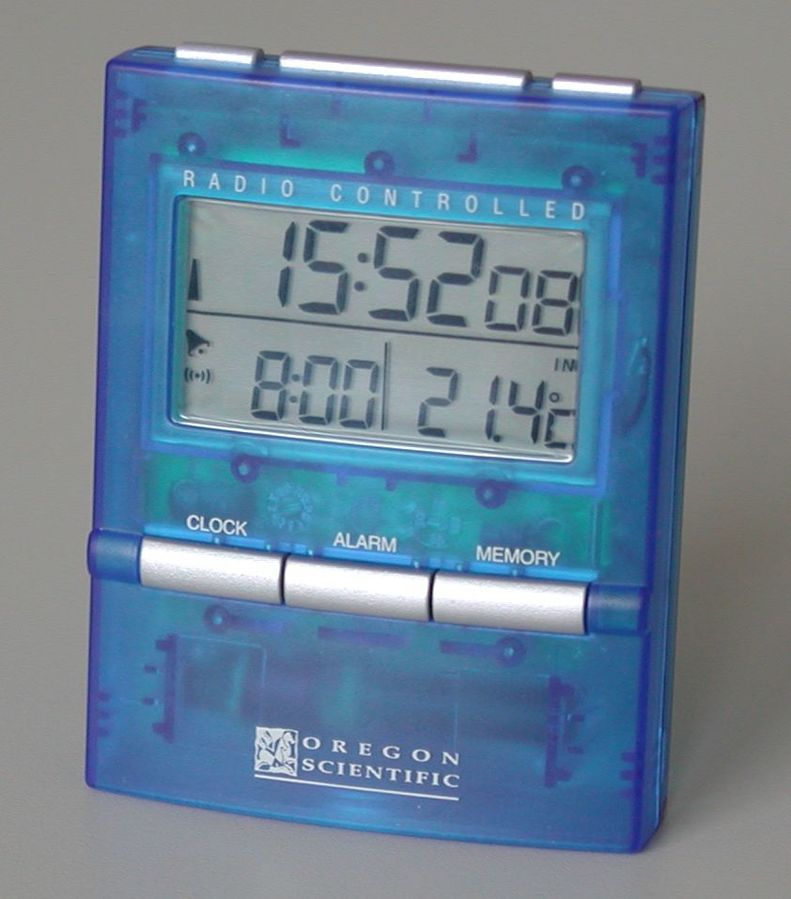
\includegraphics[width=\textwidth]{01-grundlagen/img/funkwecker}

            \column[b]{.2\textwidth}
            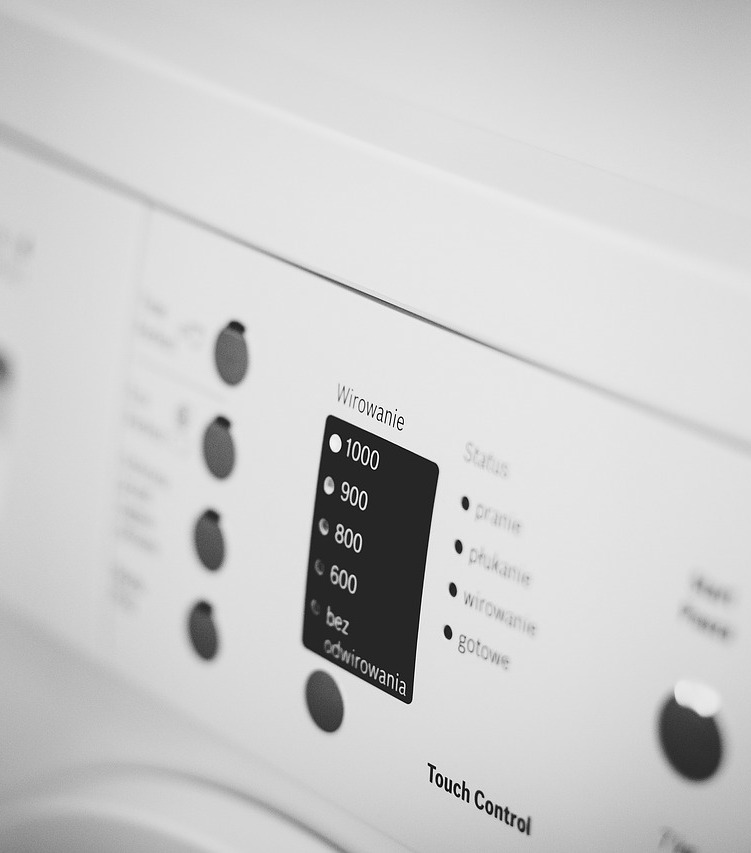
\includegraphics[width=\textwidth]{01-grundlagen/img/washing-machine-2617514_1280}

            \column[b]{.2\textwidth}
            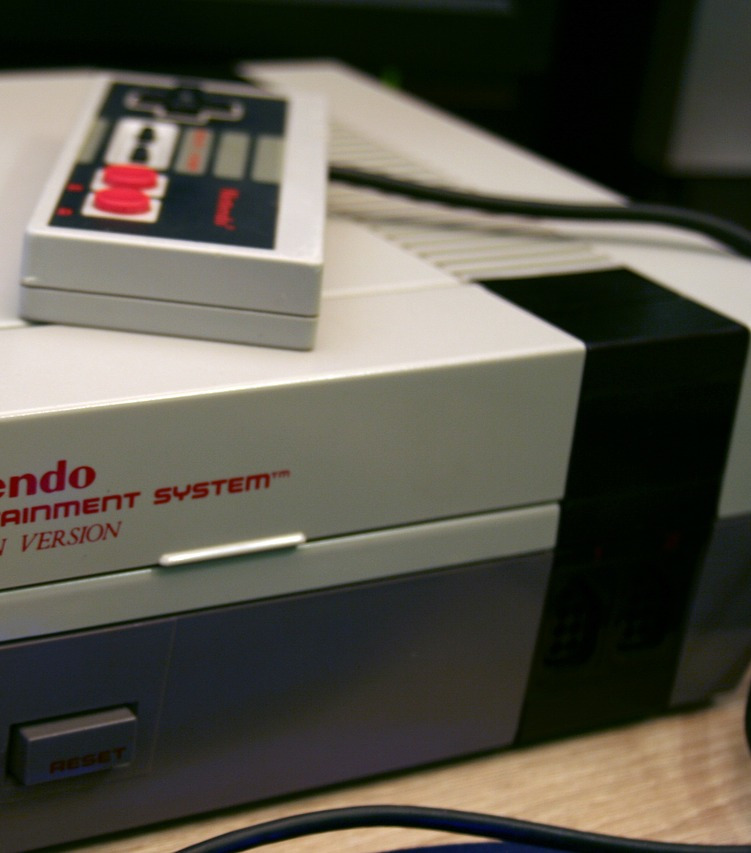
\includegraphics[width=\textwidth]{01-grundlagen/img/nes-2649705_1280}

            \column[b]{.2\textwidth}
            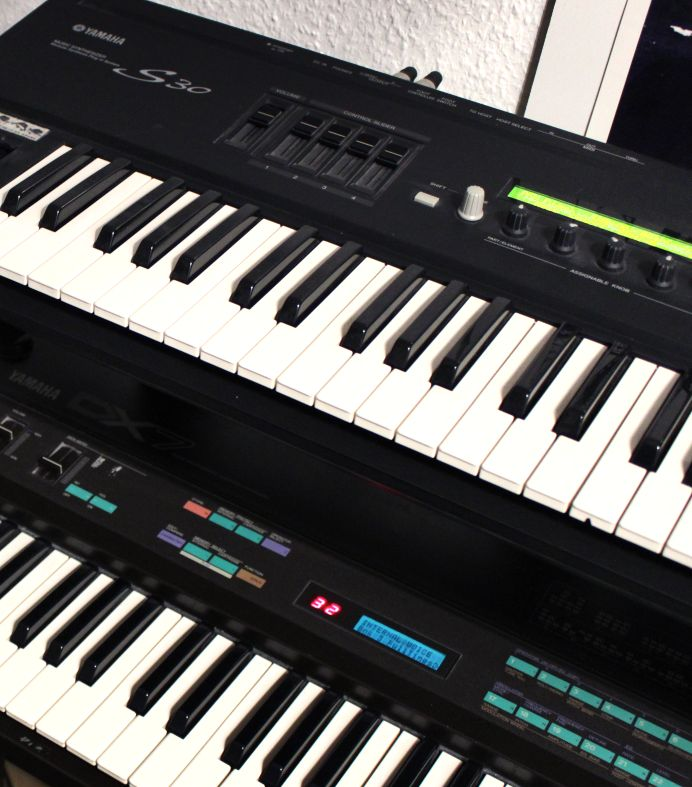
\includegraphics[width=\textwidth]{01-grundlagen/img/keyboards}

            \column[b]{.2\textwidth}
            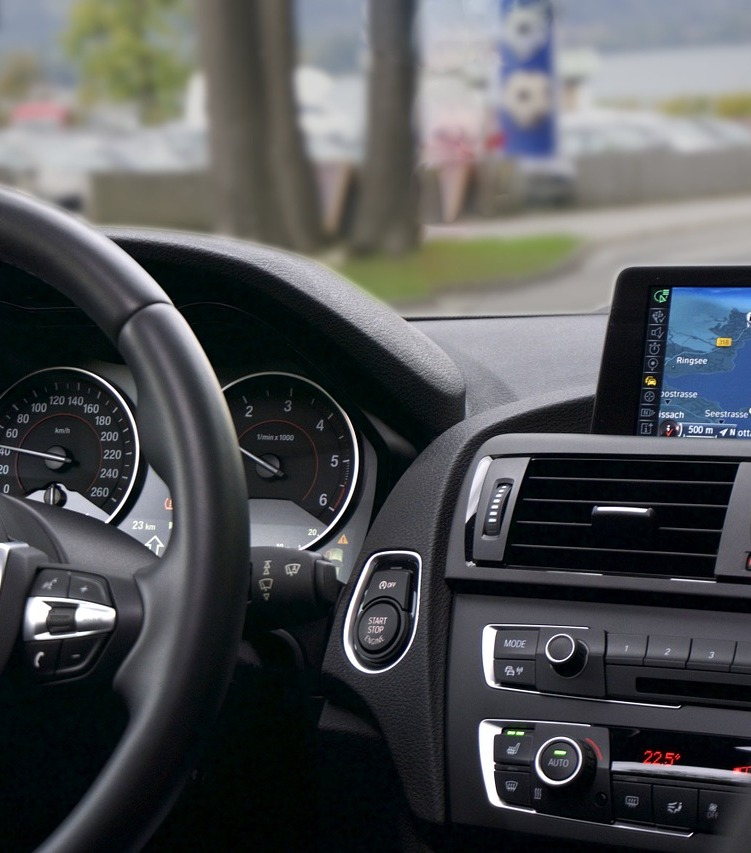
\includegraphics[width=\textwidth]{01-grundlagen/img/car-1281640_1280}
        \end{columns}
    \end{block}
\end{frame}

}
